\documentclass[10pt,a4paper]{article}
\usepackage[utf8]{inputenc}
\usepackage[german]{babel}
\usepackage{mathrsfs}
\usepackage{amsmath}
\usepackage{amsfonts}
\usepackage{amssymb}
\usepackage{amsthm}
\usepackage[left=2cm,right=2cm,top=2cm,bottom=2cm]{geometry}
\usepackage{listings}
\usepackage{graphicx}

\begin{document}

\section{Aufgabe 1}

\begin{align*}
  p(y | X, w) & = \mathcal{N}(y | Xw, \sigma^{2} I_{d})\\
  & = \frac{1}{\sqrt{(2 \pi)^{d} |\sigma^{2} I_{d}|}} e^{-\frac{1}{2}(y - Xw)^{T}(\sigma^{2} I_{d})^{-1}(y - Xw)}\\
  & = \frac{1}{\sqrt{(2 \pi \sigma^{2})^{d}}} e^{-\frac{1}{2}(y - Xw)^{T}(\frac{1}{\sigma^{2}} I_{d})(y - Xw)}
\end{align*}
\begin{align*}
  dp(y | X, w) & = d \left(\frac{1}{\sqrt{(2 \pi \sigma^{2})^{d}}} e^{-\frac{1}{2}(y - Xw)^{T}(\frac{1}{\sigma^{2}} I_{d})(y - Xw)} \right)\\
               & = \frac{1}{\sqrt{(2 \pi \sigma^{2})^{d}}} d \left(e^{-\frac{1}{2}(y - Xw)^{T}(\frac{1}{\sigma^{2}} I_{d})(y - Xw)} \right)\\
               & = \frac{e^{-\frac{1}{2}(y - Xw)^{T}(\frac{1}{\sigma^{2}} I_{d})(y - Xw)}}{\sqrt{(2 \pi \sigma^{2})^{d}}} d \left(-\frac{1}{2}(y - Xw)^{T}(\frac{1}{\sigma^{2}} I_{d})(y - Xw) \right)\\
               & = \frac{e^{-\frac{1}{2}(y - Xw)^{T}(\frac{1}{\sigma^{2}} I_{d})(y - Xw)}}{\sqrt{(2 \pi \sigma^{2})^{d}}} \left( d \left(-\frac{1}{2}(y - Xw)^{T}(\frac{1}{\sigma^{2}} I_{d}) \right)(y - Xw) - \frac{1}{2}(y - Xw)^{T}(\frac{1}{\sigma^{2}} I_{d}) d(y - Xw) \right)\\
               & = \frac{e^{-\frac{1}{2}(y - Xw)^{T}(\frac{1}{\sigma^{2}} I_{d})(y - Xw)}}{\sqrt{(2 \pi \sigma^{2})^{d}}} \left( d \left(-\frac{1}{2}(y - Xw)^{T}(\frac{1}{\sigma^{2}} I_{d}) \right)(y - Xw) + \frac{1}{2}(y - Xw)^{T}(\frac{1}{\sigma^{2}} I_{d}) X \cdot dw \right)\\
               & = \frac{e^{-\frac{1}{2}(y - Xw)^{T}(\frac{1}{\sigma^{2}} I_{d})(y - Xw)}}{\sqrt{(2 \pi \sigma^{2})^{d}}} \left( -\frac{1}{2} d(y - Xw)^{T} (\frac{1}{\sigma^{2}} I_{d})(y - Xw) + \frac{1}{2}(y - Xw)^{T}(\frac{1}{\sigma^{2}} I_{d}) X \cdot dw \right)\\
               & = \frac{e^{-\frac{1}{2}(y - Xw)^{T}(\frac{1}{\sigma^{2}} I_{d})(y - Xw)}}{\sqrt{(2 \pi \sigma^{2})^{d}}} \left( \frac{1}{2} (X \cdot dw)^{T} (\frac{1}{\sigma^{2}} I_{d})(y - Xw) + \frac{1}{2}(y - Xw)^{T}(\frac{1}{\sigma^{2}} I_{d}) X \cdot dw \right)\\
               & = \frac{e^{-\frac{1}{2}(y - Xw)^{T}(\frac{1}{\sigma^{2}} I_{d})(y - Xw)}}{2\sqrt{(2 \pi \sigma^{2})^{d}}} \left( (dw)^{T} \cdot X^{T} (\frac{1}{\sigma^{2}} I_{d})(y - Xw) + (y - Xw)^{T}(\frac{1}{\sigma^{2}} I_{d}) X \cdot dw \right)\\
               & = \frac{e^{-\frac{1}{2}(y - Xw)^{T}(\frac{1}{\sigma^{2}} I_{d})(y - Xw)}}{2\sqrt{(2 \pi \sigma^{2})^{d}}} \left( \left( (y - Xw)^{T} (\frac{1}{\sigma^{2}} I_{d})^{T} X \cdot dw \right)^{T} + (y - Xw)^{T}(\frac{1}{\sigma^{2}} I_{d}) X \cdot dw \right)\\
               & = \frac{e^{-\frac{1}{2}(y - Xw)^{T}(\frac{1}{\sigma^{2}} I_{d})(y - Xw)}}{2\sqrt{(2 \pi \sigma^{2})^{d}}} \left( (y - Xw)^{T} (\frac{1}{\sigma^{2}} I_{d})^{T} X \cdot dw + (y - Xw)^{T}(\frac{1}{\sigma^{2}} I_{d}) X \cdot dw \right) \textit{because it is scalar}\\
               & = \frac{e^{-\frac{1}{2}(y - Xw)^{T}(\frac{1}{\sigma^{2}} I_{d})(y - Xw)}}{\sqrt{(2 \pi \sigma^{2})^{d}}} \left( (y - Xw)^{T} (\frac{1}{\sigma^{2}} I_{d})^{T} X \right) \cdot dw\\
\end{align*}
So Matrix diferrential calculus tells us
\begin{equation}
  \frac{dp(y | X, w)}{dw} = \frac{e^{-\frac{1}{2}(y - Xw)^{T}(\frac{1}{\sigma^{2}} I_{d})(y - Xw)}}{\sqrt{(2 \pi \sigma^{2})^{d}}} \left( (y - Xw)^{T} (\frac{1}{\sigma^{2}} I_{d})^{T} X \right)
\end{equation}
Solving for $w$
\begin{align*}
  \frac{dp(y | X, w)}{dw} & = 0\\
  \Leftrightarrow (y - Xw)^{T} (\frac{1}{\sigma^{2}} I_{d})^{T} X & = 0\\
  \Leftrightarrow \left( (\frac{1}{\sigma^{2}} I_{d}) (y - Xw) \right)^{T} X & = 0\\
  \Leftrightarrow \frac{1}{\sigma^{2}} \left( I_{d} (y - Xw) \right)^{T} X & = 0\\
  \Leftrightarrow (y - Xw)^{T} X & = 0\\
  \Leftrightarrow (y^{T} - (Xw)^{T}) X & = 0\\
  \Leftrightarrow (y^{T} - w^{T}X^{T}) X & = 0\\
  \Leftrightarrow y^{T}X - w^{T}X^{T}X & = 0\\
  \Leftrightarrow w^{T}X^{T}X & = y^{T}X\\
  \Leftrightarrow X^{T}Xw & = X^{T}y\\
  \Leftrightarrow w & = (X^{T}X)^{-1}X^{T}y\\
\end{align*}
So the ML-estimator is $w_{MLE} = (X^{T}X)^{-1}X^{T}y$.

\section{Aufgabe 2}

\begin{equation}
  p(w) = \mathcal{N}(w | w_{0}, V_{0})
\end{equation}
\begin{equation}
  p(y | X, w) = \mathcal{N}(y | Xw, \Sigma)
\end{equation}
\begin{align*}
  p(w | X, y) & = \frac{p(y | X, w) \cdot p(w)}{p(y)}\\
              & = \frac{1}{\sqrt{(2\pi)^{D}|\Sigma|}} e^{-\frac{1}{2} (y - Xw)^{T}\Sigma^{-1}(y - Xw)} \cdot \frac{1}{\sqrt{(2\pi)^{N} |V_{0}|}} e^{-\frac{1}{2} (w - w_{0})^{T}V_{0}^{-1}(w - w_{0})}\\
              & = \frac{1}{\sqrt{(2\pi)^{D + N}|\Sigma V_{0}|}} e^{-\frac{1}{2} (y - Xw)^{T}\Sigma^{-1}(y - Xw) - \frac{1}{2} (w - w_{0})^{T}V_{0}^{-1}(w - w_{0})}\\
              & = exp \left( -\log \left( \sqrt{(2\pi)^{D + N}|\Sigma V_{0}|} \right) - \frac{1}{2} (y - Xw)^{T}\Sigma^{-1}(y - Xw) - \frac{1}{2} (w - w_{0})^{T}V_{0}^{-1}(w - w_{0}) \right)\\
              & = exp \Bigg( -\frac{1}{2}\left( (D + N) \log(2\pi)  + \log(|\Sigma V_{0}|) \right) - \frac{1}{2} (y^{T}\Sigma^{-1}y - w^{T}X^{T}\Sigma^{-1}y - y^{T}\Sigma^{-1}Xw + w^{T}X^{T}\Sigma^{-1}Xw\\& \quad + w^{T}V_{0}^{-1}w - w_{0}^{T}V_{0}^{-1}w - w^{T}V_{0}^{-1}w_{0} + w_{0}^{T}V_{0}^{-1}w_{0}) \Bigg)\\
              & = exp \Bigg( -\frac{1}{2}\left( (D + N) \log(2\pi)  + \log(|\Sigma V_{0}|) \right) - \frac{1}{2} (y^{T}\Sigma^{-1}y + w_{0}^{T}V_{0}^{-1}w_{0} - ((y^{T}\Sigma^{-1}X + w_{0}^{T}V_{0}^{-1})w)^{T}\\& \quad - (y^{T}\Sigma^{-1}X + w_{0}^{T}V_{0}^{-1})w + w^{T}(V_{0}^{-1} + X^{T}\Sigma^{-1}X)w) \Bigg)\\
              & = exp \Bigg( -\frac{1}{2}\left( (D + N) \log(2\pi)  + \log(|\Sigma V_{0}|) + y^{T}\Sigma^{-1}y + w_{0}^{T}V_{0}^{-1}w_{0} \right) + (y^{T}\Sigma^{-1}X + w_{0}^{T}V_{0}^{-1})w\\& \quad - \frac{1}{2} w^{T}(V_{0}^{-1} + X^{T}\Sigma^{-1}X)w \Bigg)\\
\end{align*}

\begin{equation}
  \Lambda = V_{0}^{-1} + X^{T}\Sigma^{-1}X
\end{equation}
\begin{equation}
  \eta^{T} = y^{T}\Sigma^{-1}X + w_{0}^{T}V_{0}^{-1}
\end{equation}
\begin{equation}
  \eta = X^{T}\Sigma^{-1}y + V_{0}^{-1}w_{0}
\end{equation}
Reordering:
\begin{equation}
  V_{n} = \Lambda^{-1} = (V_{0}^{-1} + X^{T}\Sigma^{-1}X)^{-1}
\end{equation}
\begin{equation}
  w_{n} = \Lambda^{-1}\eta = V_{n}(X^{T}\Sigma^{-1}y + V_{0}^{-1}w_{0})
\end{equation}

\section{Aufgabe 3}

\subsection{Teil b}

$d = 23$ gives the minimum test error, namely $0.3457$, over the range from $0$
to $200$.

\subsection{Teil c}

I extended the notebook with the following cell.
\begin{lstlisting}
  err(d) = begin
      phi(x) = phi_poly(x, d)
      w = wMLE(xtrain, ytrain, phi)
      mse(phi(xtrain) * w, ytrain)
  end

  ds = 1:100
  errs = map(err, ds)
  plot(layer(x = ds, y = errs, Geom.line))
\end{lstlisting}
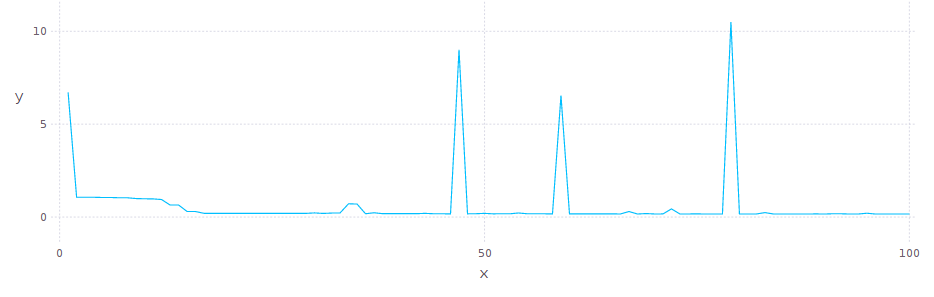
\includegraphics[width=500pt]{4_3_c.png}

\subsection{Teil d}

At first the error drops rapidly and then more slowly, until it reaches some
kind of ``minimum'' at about 20. For degrees higher than 20 the fit of the
estimation barely improves.

The most noteable feature of the plot are 3 spikes between 20 and 100. There the
error jumps up to 10. The first spike, for example, is located at polynomial
degree $47$. The mean squared errors for degrees $46, 47, 48$ are about
$0.17, 9, 0.17$.

\subsection{Teil e}

\begin{lstlisting}
  wRIDGE(x, y, phi, lambda) = begin
      X = phi(x)

      (lambda * eye(size(X)[2]) + X' * X) \ (X' * y)
  end
\end{lstlisting}

\subsection{Teil f}

\begin{lstlisting}
  findmin(map(d -> minabs(map(l -> err(d, l), linspace(0, 0.1, 100))), 1:35))
  # (0.3456978899378227,23)
\end{lstlisting}
This tells us, that the test error is quite small (namely $0.3457$) when picking degree $23$.

\begin{lstlisting}
  findmin(map(l -> err(23, l), linspace(0, 0.1, 100)))
  # (0.3456978899378227,1)
\end{lstlisting}
So the error is minimal for $\lambda = 0$.

\subsection{Teil g}

The test error is exactly the same as with MLE weights, because the test error
was minimal for $\lambda = 0$, which is just MLE regression as a special-case of
ridge regression. The weights were already very small ($< 1$ for all powers
$> 6$) without penalization, so I guess sometimes you achieve the opposite, when
reducing the weights even further.

\end{document}